\documentclass[letterpaper, 10 pt, conference]{ieeeconf} 

\usepackage[english]{babel}
\usepackage[utf8]{inputenc}
\usepackage{fullpage}
\usepackage{amsmath}
\usepackage{graphicx}
\usepackage{float}
\usepackage[colorinlistoftodos]{todonotes}
\usepackage{hyperref}
\usepackage{amssymb}
\usepackage[utf8]{inputenc}
\usepackage[english]{babel}
 
\newtheorem{theorem}{Theorem}[section]
\newtheorem{corollary}{Corollary}[theorem]
\newtheorem{lemma}[theorem]{Lemma}

\usepackage{geometry}
 \geometry{
 a4paper,
 left=17.5mm,
 right=17.5mm,
 top=20mm,
 bottom=15mm
}

\title{227A Final Project}

\author{Boying Gong (SID: 24967354)}

\begin{document}
\maketitle
\thispagestyle{empty}
\pagestyle{empty}

\onecolumn

% ========================= PART 1 =========================


\section{\textbf{Uncertainty Model}}

\subsection{Auto-Regressive Model Parameter Estimation}

\subsubsection{Formulation of the Optimization Problem} 

    Denote the number of historical data as $n$ ($n=60$ in our case). We write the auto-regressive model in the matrix form (note that the model depends on the order $p$)
	\[
	\beta_p = \begin{pmatrix} 
		\beta(p+1)  \\
		\beta(p+2)  \\
		\vdots \\
		\beta(n) 
	\end{pmatrix},
	\theta_p = \begin{pmatrix} 
		\theta(1)  \\
		\vdots \\
		\theta(p) 
	\end{pmatrix},
    \epsilon_p = \begin{pmatrix} 
		\epsilon(p+1)  \\
		\epsilon(p+2)  \\
		\vdots \\
		\epsilon(n) 
	\end{pmatrix},
	\]
    \[
    H_p = \begin{pmatrix} 
        \beta(p)   & \beta(p-1) & \cdots & \beta(1)   \\
        \beta(p+1) & \beta(p)   & \cdots & \beta(2)   \\
        \vdots     & \vdots     & \ddots & \vdots     \\
        \beta(n-1) & \beta(n-2) & \cdots & \beta(n-p) \\
    \end{pmatrix}.
    \]
	\[ 
	\beta_p=H_p\theta_p+\sigma_p\epsilon_p, \quad ||\epsilon_p||_\infty \leq 1.
	\]

	Now we estimate the values of $\theta_p$ and $\sigma_p$ by minimizing the infinity norm of the error
	\[
	\min_{\hat{\theta}_p}||\beta_p-\hat{\beta}_p||_\infty, \quad
    \text{s.t. }\hat{\beta}_p = H_p\hat{\theta}_p,
	\]
	This is equivalent to the following LP problem, where we use $\hat{\sigma}$ as an estimate of $\sigma$.
	\begin{equation}\label{eq:ar_opt} 
	\min_{\hat{\theta}_p, \hat{\sigma}_p}\hat{\sigma}_p, \quad
    \text{s.t. }\hat{\beta}_p=H_p\hat{\theta}_p,|\beta_p-\hat{\beta}_p|\preceq\hat{\sigma}_p.
	\end{equation}

\subsubsection{Order Selection for the Auto-Regressive Model} 

    The order $p$ of the autoregressive model needs to be determined. Because our goal is to predict the cash flow requirement in the next 6 months, prediction error is important. We use cross-validation on a rolling basis to calculate the prediction error for $1\leq p\leq 30$. The cross-validation procedure is described as follows.\cite{cvTs} For each $p$, 
    \begin{enumerate}
    	\item Fit the model to the data $\beta_1,\cdots,\beta_t$ and let $\hat{\beta}^{(t)}_{t+1},\cdots,\hat{\beta}^{(t)}_{t+6}$ denote the forecasts of the next 6 months. Then compute the error ($e^{(t)}_{t+i} = \beta_{t+i}- \hat{\beta}^{(t)}_{t+i}$) for the forecast observations. 
        \item Repeat step 1 for $t=n-15,\cdots,n-6$ (10-fold). 
        \item Compute : (I) the proportion of absolute error $|e^{(t)}_{t+i}|$ that are greater than the $\sigma$ estimation $|\sigma^{(t)}|$. We call it out-of-bound error.
        (II) MAE (Mean Absolute Error) from the errors $e^{(t)}_{t+i}, t=n-15,\cdots,n-6,i=1,\cdots,6$. 
    \end{enumerate}
    Then, we choose $p$ with the smallest out-of-bound error. For $p$'s with the same out-of-bound error, we choose $p$ with the smallest MAE.

\subsubsection{Results}

     \begin{figure*}
        \centering
        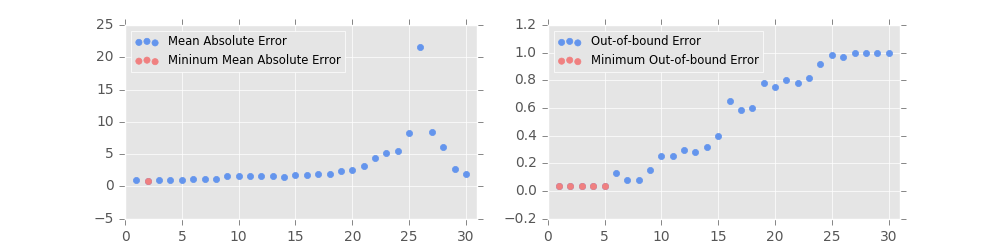
\includegraphics[width=0.8\textwidth]{cv.png}
        \caption{Cross-validation Results for Order selection}
        \label{fig:cv_result}
    \end{figure*} 

    The cross-validation results are shown in Figure \ref{fig:cv_result}, the minimum  out-of-bound error and MAE are both attained when $p=2$. We use $p=2$ to solve the optimization problem (\ref{eq:ar_opt}). The solution is
    \[\sigma^* = 3.24341242878, \theta^*_1 = 0.44904669, \theta^*_2 = 0.53272938.\]
    And the corresponding auto-regressive model is given by
    \begin{equation}\label{eq:ar-est}
    	\beta(t+1) = \theta_1^*\beta(t) + \theta_2^*\beta(t-1)+\sigma^*\epsilon(t+1),
    \end{equation}
    \[\quad|\epsilon(t+1)|\leq 1.\]

\subsection{Uncertainty Model}

    Let $u = (\epsilon(t+1), \cdots, \epsilon(t+T))^T$. With the auto-regressive model (\ref{eq:ar-est}), $\hat{b}(t)$ and $B(t)$ can be expressed as a function of $\beta(t), \beta(t-1), \theta_1^*, \theta_2^*$ and $\sigma^*$ using recursive substitution. The derivation is given in Appendix \ref{apx:recursive substitution}. From the historical data, $\beta(t) = 1.4880$ and $\beta(t-1)=3.5112$. The numerical value is given below
    \[
	   \hat{b}(t) = 
        \begin{pmatrix}
    	2.539 & 1.933 & 2.220 & 2.027 & 2.093 & 2.020
	   \end{pmatrix}^T,
    \]
    \[
	   B(t) = 
        \begin{pmatrix}
    	   3.243 & 0 & 0 & 0 & 0 & 0 \\
            1.456 & 3.243 & 0 & 0 & 0 & 0 \\
            2.382 & 1.456 & 3.243 & 0 & 0 & 0 \\
            1.846 & 2.382 & 1.456 & 3.243 & 0 & 0 \\
            2.098 & 1.846 & 2.382 & 1.456 & 3.243 & 0 \\
            1.925 & 2.098 & 1.846 & 2.382 & 1.456 & 3.243
        \end{pmatrix}.
    \]


% ========================= PART 2 =========================

\section{\textbf{Decision Making}}

% ================== Naive Strategy ==================

\subsection{Naive Strategy}

    Let $C_{initial} = 70.3$ be the amount that the company has at the beginning of the horizon, and $l = (C_{initial}, 0, 0, 0, 0, 0)$. Let $x=(x_{cash}, x_{cp}, x_{cre}), x_{cash}\in\mathbb{R}^6, x_{cp}\in\mathbb{R}^3, x_{cre}\in\mathbb{R}^5$. In the naive strategy, we assume the future liability be $\hat{b(t)}$ without error. 
    
    In January ($i = 1$), the company can draw an amount $x_{cre}(1)$ from its line of credit and issue an amount $x_{cp}(1)$ of commercial paper. Together with the initial asset $C_{initial}$, $x_{cre}(1)+x_{cp}(1)+C_{initial}$ will be used for investment and meeting the liabilities. The balance equation is as follows, 
    \[
        x_{cre}(1)+x_{cp}(1)+C_{initial}-x_{cash}(1) = b_1
    \]
    Similarly, we can get the equation for other months and obtain the following LP formulation:
    \[
        \begin{split}
            \max_{x} \quad & x_{cash}(6) \\
            \text{s.t.} \quad 
            & x_{cre}(1) + x_{cp}(1)+C_{initial}-x_{cash}(1) = b_1 \\
            & x_{cre}(2) + x_{cp}(2) -1.01x_{cre}(1) + 1.003x_{cash}(1) -x_{cash}(2) = b_2 \\
            & x_{cre}(3) + x_{cp}(3) -1.01x_{cre}(2) + 1.003x_{cash}(2) -x_{cash}(3) = b_3 \\
            & x_{cre}(4) - 1.02x_{cp}(1) - 1.01x_{cre}(3) + 1.003x_{cash}(3) - x_{cash}(4) = b_4 \\
            & x_{cre}(5) - 1.02x_{cp}(2) - 1.01x_{cre}(4) + 1.003x_{cash}(4) - x_{cash}(5) = b_5 \\
            & - 1.02x_{cp}(3) - 1.01x_{cre}(5) + 1.003x_{cash}(5) - x_{cash}(6) = b_6 \\
            & 0 \leq x_{cre}(i) \leq 1, i = 1, \cdots, 5.\\
            & x_{cp} \geq 0, i = 1, 2, 3.\\
            & x_{cash}(i)\geq 0, i = 1, \cdots, 6.
        \end{split}
    \]
    Write this in LP format:
    \[
        \min_x c^Tx: Ax+l\geq\hat{b}(t), 0\leq x\leq \bar{x} 
    \]
    The maximization of the amount of cash at the end of the period is $58.4301$. The optimal strategy is 
    \[
        x_{cash} = 
        \begin{pmatrix}
        7.761 & 66.032 & 64.010 & 62.175 & 60.269 & 58.430
        \end{pmatrix}^T,
    \]
    $x_{cp}$ and $x_{cre}$ equal to 0.
    
    The results show that if the company have sufficient amount of initial asset, say 70.3 million, the naive strategy will not turn to credit line nor commercial paper.

    Figure \ref{fig:naive} shows that as we decrease the amount of initial funds, the optimal amount for credit line $X_{cre}$ and commercial paper $X_{cp}$ will stay 0. The optimal value of excess funds to be invested $X_{cash}$ will decrease linearly. This is because it is the only source to cover the liability and the constraints are linear. When the initial funds drops below 12.739 million, the problem will become infeasible.
    \begin{figure*}
	   \centering
	   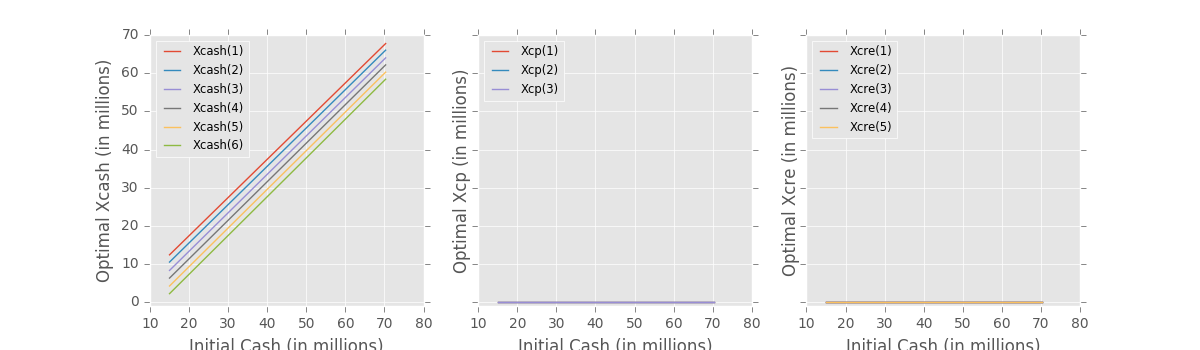
\includegraphics[width=0.7\textwidth]{naive.png}
        \caption{Optimal naive strategy for difference initial assets}
        \label{fig:naive}
    \end{figure*}  

% ================== Robust Strategy ==================

\subsection{Robust Strategy}

    We now consider the robust counterpart of the problem
    \begin{equation}\label{eq:robust}
	   \min_x c^Tx: Ax+l\geq b(t), b(t)\in\mathcal{U}(t) ,0\leq x\leq \bar{x}
    \end{equation}
    The constrains $Ax+l\geq b(t), b(t)\in\mathcal{U}(t)$ can be written as follows based on the autoregressive model assumption
    \[\begin{split}
        & Ax+l\geq \hat{b}(t) + B(t)u, \forall ||u||_\infty \leq 1 \\
        \iff & Ax+l\geq \hat{b}(t) + \max_{||u||_\infty \leq 1}B(t)u \\
        \iff & Ax+l\geq \hat{b}(t) + |B(t)|\textbf{1}
    \end{split}\]
    Thus, we can formulate the model as
    \begin{equation}\label{eq:robust_final}
        \min_x c^Tx: Ax+l\geq \hat{b}(t) + |B(t)|\textbf{1}, 0\leq x\leq \bar{x} 
    \end{equation}
    The optimal objective value is $10.2471$. The optimal strategy is 
    \[
        x_{cash} = 
        \begin{pmatrix}
        64.518 & 58.079 & 48.951 & 38.144 & 25.141 & 10.247
        \end{pmatrix}^T,
    \]
    $x_{cp}$ and $x_{cre}$ equals to 0. The results shows that if the company have sufficient amount of initial asset, the robust strategy will not turn to credit line nor commercial paper. The robust strategy is much more conservative than the naive strategy in that it uses less cash for investment and more for covering the liability.

    Figure \ref{fig:robust} shows the robust counterpart of Figure \ref{fig:naive}. As we decrease the amount of initial funds, the optimal amount for credit line $X_{cre}$ and commercial paper $X_{cp}$ will stay 0 as well. The optimal value of excess funds to be invested $X_{cash}$ will decrease linearly. When the initial funds drops below 60.205 million, the problem will become infeasible.
    \begin{figure*}
	   \centering
	   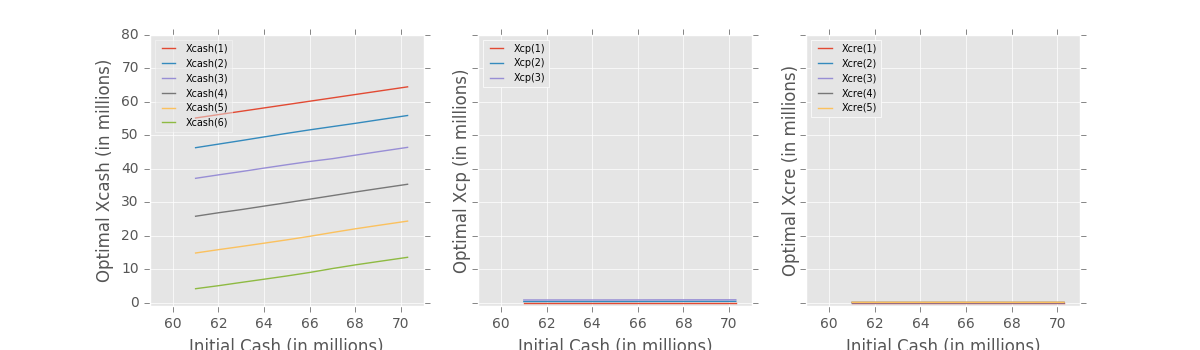
\includegraphics[width=0.7\textwidth]{robust.png}
        \caption{Optimal robust strategy for difference initial assets}
        \label{fig:robust}
    \end{figure*}  

% ========= Affine Strategy =========

\subsection{Affine Strategy}

    Assume that at each time $t$, the information in previous time points (up to $t-1$) are available. We further assume that the decision variables are linear functions of previous information.
    \[
        x_{cash}(u) = x_{cash} + X_{cash}u,
    \]
    \[ 
        x_{cp}(u) = x_{cp} + X_{cp}u,
    \]
    \[ 
        x_{cre}(u) = x_{cre} + X_{cre}u.
    \]
    Let $X=(X_{cash}^T, X_{cp}^T, X_{cre}^T)^T$, the optimization problem can be formulated as 
    \[\begin{split}
	   \max_x\ & \min_{u:||u||_\infty \leq 1} c^Tx(u) \\
        \text{s.t. } & X_{cash},  X_{cp}, X_{cre} \text{ strictly lower-triangular,}\\
        & A(x + Xu) + l\geq b(t) + B(t)u,\forall b(t) \in \mathcal{U},\\
        & 0\leq x+Xu \leq \bar{x}.
    \end{split}\]
    The constraint $A(x + Xu) + l\geq b(t) + B(t)u,\forall b(t) \in \mathcal{U}$ can be written as follows
    \[\begin{split}
        & A(x + Xu) + l\geq \hat{b}(t) + B(t)u,\forall ||u||_\infty\leq 1 \\
        \iff & Ax+l\geq \hat{b}(t) + (B(t)-AX)u, \forall ||u||_\infty \leq 1 \\
        \iff & Ax+l\geq \hat{b}(t) + \max_{||u||_\infty \leq 1}(B(t)-AX)u \\
        \iff & Ax+l\geq \hat{b}(t) + |(B(t)-AX)|\textbf{1}
    \end{split}\]
    The objective function $\min_{u:||u||_\infty \leq 1} c^Tx(u)$ is equivalent to
    \[\begin{split}
    & c^Tx - \max_{u:||u||_\infty \leq 1} c^TX(-u) \\
    = & c^Tx - ||X^Tc||_1
    \end{split}\]
    Thus, we can formulate the affine strategy as the following LP problem
    \[\begin{split}
	   \max_{x, X}\ & c^Tx - ||X^Tc||_1  \\
        \text{s.t. } & X_{cash},  X_{cp}, X_{cre} \text{ strictly lower-triangular,}\\
        & Ax + l\geq  \hat{b}(t) + |B(t) - AX|\textbf{1}, 0\leq x+Xu \leq \bar{x}.
    \end{split}\]

    The optimal solution is 
    \[\begin{split}
        x_{cash} = &
        \begin{pmatrix}
        64.52 &  55.96 & 46.45 & 35.43 & 24.45 & 13.62
        \end{pmatrix}^T, \\
        x_{cp} = &
        \begin{pmatrix}
        0 & 0.467 & 0.929
        \end{pmatrix}^T, \\
        x_{cre} = &
        \begin{pmatrix}
        0 & 0.061 & 0.104 & 0.148 & 0.179
        \end{pmatrix}^T, \\
        X_{Cash} = &
        \begin{pmatrix}
            0     &  0     &    0   &   0   &  0       &  0 \\
            2.12  &  0     &    0   &   0   &  0       &  0 \\
            1.28  &  1.23  &    0   &   0   &  0       &  0 \\
            0.83  &  0.82  &   1.07 &   0   &  0       &  0 \\
            0.13  &  0.12  &   0.12 & 0.34  &  0       &  0 \\
            -0.58 &  -0.65 &  -0.71 & -0.80 &  -0.63   &  0
        \end{pmatrix}, \\
        X_{Cp} = &
        \begin{pmatrix}
            0       &  0       &    0   &   0   &  0   &  0 \\
            -0.467  &  0       &    0   &   0   &  0   &  0 \\
            -0.4656 &  -0.4635 &    0   &   0   &  0   &  0 \\
        \end{pmatrix}^T, \\
        X_{Cre} = &
        \begin{pmatrix}
            0      &  0      &    0   &   0    &  0  &  0 \\
            -0.061 &  0      &    0   &   0    &  0  &  0 \\
            -0.052 &  -0.052 &    0   &   0    &  0  &  0 \\
            -0.049 &  -0.050 & -0.050 &   0    &  0  &  0 \\
            -0.045 &  -0.045 & -0.045 & -0.045 &  0  &  0
        \end{pmatrix}^T.
    \end{split}\]
    \begin{figure*}
       \centering
       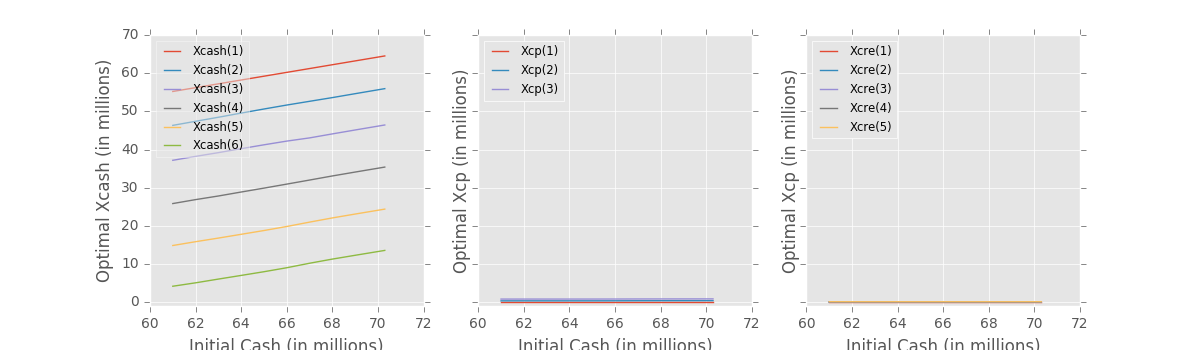
\includegraphics[width=0.7\textwidth]{affine.png}
        \caption{Optimal affine strategy for difference initial assets}
        \label{fig:affine}
    \end{figure*}
    TO BE COMPLETED TO BE COMPLETED TO BE COMPLETED TO BE COMPLETED TO BE COMPLETED TO BE COMPLETED TO BE COMPLETED TO BE COMPLETED TO BE COMPLETED TO BE COMPLETED TO BE COMPLETED TO BE COMPLETED TO BE COMPLETED TO BE COMPLETED TO BE COMPLETED TO BE COMPLETED TO BE COMPLETED TO BE COMPLETED TO BE COMPLETED TO BE COMPLETED TO BE COMPLETED TO BE COMPLETED TO BE COMPLETED TO BE COMPLETED TO BE COMPLETED TO BE COMPLETED TO BE COMPLETED TO BE COMPLETED TO BE COMPLETED TO BE COMPLETED TO BE COMPLETED TO BE COMPLETED TO BE COMPLETED TO BE COMPLETED TO BE COMPLETED TO BE COMPLETED TO BE COMPLETED TO BE COMPLETED TO BE COMPLETED TO BE COMPLETED 

% ========= Relative Robust Strategy =========

    \begin{figure*}
       \centering
       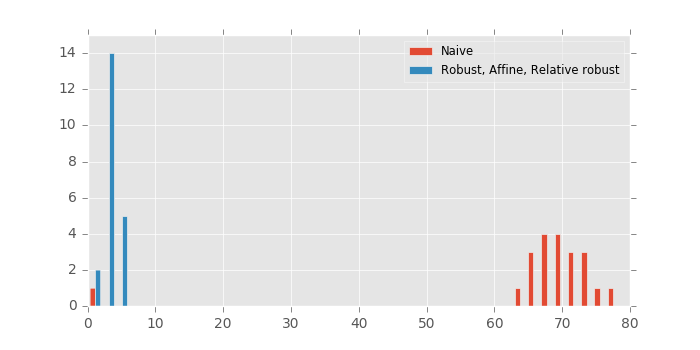
\includegraphics[width=0.45\textwidth]{regret.png}
        \caption{Regret histogram of more test data}
        \label{fig:regret}
    \end{figure*}

\subsection{Relative Robust Strategy}

    For the relative robust strategy, we consider minimizing the maximum regret for problem (\ref{eq:robust}). The regret function measures the difference between the performance of the solution with and without the full knowledge of the future. Assume we choose $x$ as decision vector, $u$ is the vector of realized parameter values and $x^*(u)$ is the optimal decision vector if $u$ is available. The regret associated with having chosen $x$ rather than $x^*(u)$ as decision vector is defined as follows,
    \[
        r(x, u) =  c^Tx - c^Tx^*(u).
    \]
    The regret will always be greater than 0. The relative robust problem of minimizing the maximum regret can be formulated as follows
    \[\begin{split}
        \min_{x} & \big\{ \quad\max_{||u||_\infty\leq 1} \big\{c^Tx - 
        \min_{\{y:Ay+l\geq \hat{b}(t)+B(t)u, 0\leq y\leq \bar{x} \}} c^Ty\big\}\big\}. \\
        \text{s.t. } & Ax+l\geq \hat{b}(t) + B(t)u, \forall ||u||_\infty\leq 1, \\
        & 0\leq x\leq \bar{x}.
    \end{split}\]
    Introducing a slack variable $\gamma$ that expresses an upper bound on the regret, we can equivalently reformulate this problem as follows,
    \[\begin{split}
        \min_{x, y, \gamma}\ & \gamma \\
        \text{s.t. } 
        & Ax+l\geq \hat{b}(t) + B(t)u, \forall ||u||_\infty\leq 1,  \\
        & 0\leq x\leq \bar{x}, \\
        & \gamma \geq c^Tx + \max_{||u||_\infty\leq 1} \big\{
        \max_{\{y:Ay+l\geq \hat{b}(t)+B(t)u, 0\leq y\leq \bar{x} \}} - c^Ty\big\}.
    \end{split}\]
    Similar to the robust problem and the affine problem, this can also be expressed as{} follows
    \begin{equation}\label{eq:relative}\begin{split}
        \min_{x, y, \gamma}\ & \gamma \\
        \text{s.t. } 
        & Ax+l\geq \hat{b}(t) + |B(t)|\textbf{1}, \\
        & 0\leq x\leq \bar{x}, \\
        & \gamma \geq c^Tx + \max_{||u||_\infty\leq 1} \big\{
        \max_{\{y:Ay+l\geq \hat{b}(t)+B(t)u, 0\leq y\leq \bar{x} \}} - c^Ty\big\}.
    \end{split}\end{equation}
    Notice that the set $\{||u||_\infty \leq 1\}$ can be expressed as a convex hull of a finite number of extreme scenarios, namely
    \[\{||u||_\infty \leq 1\} = \text{conv}(\{u^{[i]}, i = 1, \cdots, 2^T\})\]
    We have the following lemma:

    \begin{lemma}
        The following are equivalent, 
        \begin{enumerate}
            \item $-c^Tx+\gamma \geq
            \max_{\{y:Ay+l\geq \hat{b}(t)+B(t)u, 0\leq y\leq \bar{x} \}} - c^Ty,$\\ $\forall ||u||_\infty\leq 1,$
            \item $-c^Tx+\gamma \geq
            \max_{\{y:Ay+l\geq \hat{b}(t)+B(t)u^{[i]}, 0\leq y\leq \bar{x} \}} - c^Ty,$\\$ i = 1, \cdots, 2^T$.
        \end{enumerate}
    \end{lemma}
    \emph{Proof. } For the proof, please refer to Corollary 4.1 in \cite{hauser2013relative}.

    Thus, problem (\ref{eq:relative}) is equivalent to 
    \begin{equation}\label{eq:relative_final}\begin{split}
        \min_{x, y, \gamma}\ & \gamma \\
        \text{s.t. } 
        & Ax+l\geq \hat{b}(t) + |B(t)|\textbf{1}, \\
        & 0\leq x\leq \bar{x}, \\
        & \gamma \geq c^Tx + g(i),  i = 1, \cdots, 2^T, \\
        & g(i) = \max_{\{y:Ay+l\geq \hat{b}(t)+B(t)u^{[i]}, 0\leq y\leq \bar{x} \}} - c^Ty.
    \end{split}\end{equation}

    We can solve problem (\ref{eq:relative_final}) with a two-step procedure where we first solve an LP problem for $y$ (that is, solve $g(i)$), and then solve the LP problem for $x$ and $\gamma$.

    Notice that the optimal solution of (\ref{eq:relative}) is equal to the optimal solution of the robust problem (\ref{eq:robust_final}). To see this fact, let $g = \max_i g(i)$. $g$ can be treated as a constant since $g(i)$ can be solved explicitly. Then (\ref{eq:relative}) is quivalent to the following
    \[\begin{split}
        \min_{x, y}\ & c^Tx + g \\
        \text{s.t. } 
        & Ax+l\geq \hat{b}(t) + |B(t)|\textbf{1}, \\
        & 0\leq x\leq \bar{x}.
    \end{split}\]
    which is the same as (\ref{eq:relative}). Note that the robust solution and relative robust optimization problem does not usually equivalent to each other without the linearity of object and contraints function. 

% ========================= PART 3 =========================

\section{\textbf{Evaluation Metrics}}

\subsection{Test Data}

    \begin{table}[H]
        \begin{tabular}{|l|p{1.3cm}|p{1.3cm}|p{1.3cm}|p{1.3cm}|}
        \hline
        & Naive & Robust & Affine & Relative Robust \\ 
        \hline
        Regret & 8.71 & 56.90 & 52.97 & 56.90 \\
        \hline
        \end{tabular}
        \caption{Regret for test data}
    \end{table}

\subsection{More Test Data}



\bibliographystyle{plain}
\bibliography{Proof_of_Correctness.bib}

\clearpage
\newpage
\appendix

% ======================= Appendix A =======================
\section{Appendix: AR(2) Recursive Substitution}\label{apx:recursive substitution}

Let $u = (\epsilon(t+1), \cdots, \epsilon(t+T))^T$. With the auto-regressive model (\ref{eq:ar-est}), $\hat{b}(t)$ and $B(t)$ can be expressed as a function of $\beta(t), \beta(t-1), \theta_1^*, \theta_2^*$ and $\sigma^*$ using recursive substitution. 
\[\beta(t+1) = \theta_1\beta(t)+\theta_2\beta(t-1)+\sigma\epsilon(t+1)\]
\[\begin{split}
	\beta(t+2) 
    = & \theta_1\beta(t+1)+\theta_2\beta(t)+\sigma\epsilon(t+2) \\
    = & \theta_1[\theta_1\beta(t)+\theta_2\beta(t-1)+\sigma\epsilon(t+1)]+
    	\theta_2\beta(t)+\sigma\epsilon(t+2) \\
    = & (\theta_1^2+\theta_2)\beta(t)+\theta_1\theta_2\beta(t-1)+
    	\theta_1\sigma\epsilon(t+1)+\sigma\epsilon(t+2)
\end{split}\]
\[\begin{split}
	\beta(t+3) 
    = & \theta_1\beta(t+2)+\theta_2\beta(t+1)+\sigma\epsilon(t+3) \\
    = & \theta_1\big[(\theta_1^2+\theta_2)\beta(t)+\theta_1\theta_2\beta(t-1)+
    	\theta_1\sigma\epsilon(t+1)+\sigma\epsilon(t+2)\big]+ \\
      & \theta_2\big[\theta_1\beta(t)+\theta_2\beta(t-1)+\sigma\epsilon(t+1)\big]+\sigma\epsilon(t+3) \\
    = & (\theta_1^3+2\theta_1\theta_2)\beta(t) + (\theta_1^2\theta_2+\theta_2^2)\beta(t-1) + \\
      &	(\theta_1^2+\theta_2)\sigma\epsilon(t+1) + \theta_1\sigma\epsilon(t+2) +
        \sigma\epsilon(t+3)
\end{split}\]
\[\begin{split}
	\beta(t+4) 
    = & \theta_1\beta(t+3)+\theta_2\beta(t+2)+\sigma\epsilon(t+4) \\
    = & \theta_1\big[ (\theta_1^3+2\theta_1\theta_2)\beta(t) + (\theta_1^2\theta_2+\theta_2^2)\beta(t-1) + \\
      &	(\theta_1^2+\theta_2)\sigma\epsilon(t+1) + \theta_1\sigma\epsilon(t+2) +
        \sigma\epsilon(t+3)\big]+\\
      & \theta_2\big[ (\theta_1^2+\theta_2)\beta(t)+\theta_1\theta_2\beta(t-1)+
    	\theta_1\sigma\epsilon(t+1)+\sigma\epsilon(t+2)\big]+\sigma\epsilon(t+4) \\
    = & (\theta_1^4+3\theta_1^2\theta_2+\theta_2^2)\beta(t)+
    	(\theta_1^3\theta_2+2\theta_1\theta_2^2)\beta(t-1)+\\
       & (\theta_1^3+2\theta_1\theta_2)\sigma\epsilon(t+1)+(\theta_1^2+\theta_2)\sigma\epsilon(t+2)+\theta_1\sigma\epsilon(t+3)+\sigma\epsilon(t+4)
\end{split}\]
\[\begin{split}
	\beta(t+5) = & \theta_1\beta(t+4)+\theta_2\beta(t+3)+\sigma\epsilon(t+5) \\
    = & \theta_1\big[(\theta_1^4+3\theta_1^2\theta_2+\theta_2^2)\beta(t)+
    	(\theta_1^3\theta_2+2\theta_1\theta_2^2)\beta(t-1)+\\
      & (\theta_1^3+2\theta_1\theta_2)\sigma\epsilon(t+1)+(\theta_1^2+\theta_2)\sigma\epsilon(t+2)+\theta_1\sigma\epsilon(t+3)+\sigma\epsilon(t+4)\big]+\\
      & \theta_2\big[(\theta_1^3+2\theta_1\theta_2)\beta(t) + (\theta_1^2\theta_2+\theta_2^2)\beta(t-1) + \\
      &	(\theta_1^2+\theta_2)\sigma\epsilon(t+1) + \theta_1\sigma\epsilon(t+2) +
        \sigma\epsilon(t+3)\big]+\sigma\epsilon(t+5) \\
  	= & (\theta_1^5+4\theta_1^3\theta_2+3\theta_1\theta_2^2)\beta(t) +
        (\theta_1^4\theta_2+3\theta_1^2\theta_2^2+\theta_2^3)\beta(t-1) + \\
      &(\theta_1^4+3\theta_1^2\theta_2+\theta_2^2)\sigma\epsilon(t+1)+(\theta_1^3+2\theta_1\theta_2)\sigma\epsilon(t+2)+(\theta_1^2+\theta_2)\sigma\epsilon(t+3)+\theta_1\sigma\epsilon(t+4)+\sigma\epsilon(t+5)
\end{split}\]
\[\begin{split}
	\beta(t+6) =
      & \theta_1\beta(t+5)+\theta_2\beta(t+4)+\sigma\epsilon(t+6) \\
    = & \theta_1\big[(\theta_1^5+4\theta_1^3\theta_2+3\theta_1\theta_2^2)\beta(t) +
        (\theta_1^4\theta_2+3\theta_1^2\theta_2^2+\theta_2^3)\beta(t-1)\\
      & (\theta_1^4+3\theta_1^2\theta_2+\theta_2^2)\sigma\epsilon(t+1)+(\theta_1^3+2\theta_1\theta_2)\sigma\epsilon(t+2)+(\theta_1^2+\theta_2)\sigma\epsilon(t+3)+\theta_1\sigma\epsilon(t+4)+\sigma\epsilon(t+5)\big]+\\
      & \theta_2\big[(\theta_1^4+3\theta_1^2\theta_2+\theta_2^2)\beta(t)+
    	(\theta_1^3\theta_2+2\theta_1\theta_2^2)\beta(t-1)+\\
      & (\theta_1^3+2\theta_1\theta_2)\sigma\epsilon(t+1)+(\theta_1^2+\theta_2)\sigma\epsilon(t+2)+\theta_1\sigma\epsilon(t+3)+\sigma\epsilon(t+4)\big]+\sigma\epsilon(t+6) \\
    = & (\theta_1^6+5\theta_1^4\theta_2+6\theta_1^2\theta_2^2+\theta_2^3)\beta(t) +
        (\theta_1^5\theta_2+4\theta_1^3\theta_2^2+3\theta_1\theta_2^3)\beta(t-1)\\
      & (\theta_1^5+4\theta_1^3\theta_2+3\theta_1\theta_2^2)\sigma\epsilon(t+1)+(\theta_1^4+3\theta_1^2\theta_2+\theta_2^2)\sigma\epsilon(t+2)+ \\
      & (\theta_1^3+2\theta_1\theta_2)\sigma\epsilon(t+3)+(\theta_1^2+\theta_2)\sigma\epsilon(t+4)+\theta_1\sigma\epsilon(t+5)+\sigma\epsilon(t+6)
\end{split}\]

Express the previous equation in the matrix form, we get

\[
	\hat{b}(t) = 
    \begin{pmatrix}
    	\theta_1 & \theta_2\\
		\theta_1^2+\theta_2 & \theta_1\theta_2 \\
        \theta_1^3+2\theta_1\theta_2 & \theta_1^2\theta_2+\theta_2^2 \\
        \theta_1^4+3\theta_1^2\theta_2+\theta_2^2 & 
    	\theta_1^3\theta_2+2\theta_1\theta_2^2 \\
        \theta_1^5+4\theta_1^3\theta_2+3\theta_1\theta_2^2 & 
        \theta_1^4\theta_2+3\theta_1^2\theta_2^2+\theta_2^3 \\
        \theta_1^6+5\theta_1^4\theta_2+6\theta_1^2\theta_2^2+\theta_2^3 & 
        \theta_1^5\theta_2+4\theta_1^3\theta_2^2+3\theta_1\theta_2^3 \\
	\end{pmatrix}
    \begin{pmatrix}
		\beta(t) \\
        \beta(t-1)
	\end{pmatrix}
\]
\[
	B(t) = 
    \sigma\begin{pmatrix}
    	1 & 0 & 0 & 0 & 0 & 0\\
    	\theta_1 & 1 & 0 & 0 & 0 & 0\\
    	\theta_1^2+\theta_2 & \theta_1 & 1 & 0 & 0 & 0\\
        \theta_1^3+2\theta_1\theta_2 & \theta_1^2+\theta_2 & \theta_1 & 1 & 0 & 0\\
    	\theta_1^4+3\theta_1^2\theta_2+\theta_2^2 & 
        \theta_1^3+2\theta_1\theta_2 & \theta_1^2+\theta_2 & \theta_1 & 1 & 0\\
    	\theta_1^5+4\theta_1^3\theta_2+3\theta_1\theta_2^2 &
        \theta_1^4+3\theta_1^2\theta_2+\theta_2^2 & 
        \theta_1^3+2\theta_1\theta_2 & \theta_1^2+\theta_2 & \theta_1 & 1
    \end{pmatrix}
\]

\end{document}
